\newcommand{\hdistance}{10em}
\newcommand{\vdistance}{8.5em}
\newcommand{\imagewidth}{3em}
\newcommand{\relatedtotext}{«related to»}
\newcommand{\usestext}{«uses»}
\newcommand{\knowsabouttext}{«knows about»}

\begin{tikzpicture}[
    tool/.style={anchor=center, align=center, font=\footnotesize},
    role/.style={anchor=north, align=center, font=\footnotesize},
    relation/.style={consistency relation},
    uses/.style={consistency execution},
    knows/.style={-latex, color=darkorange},
]

\node[draw, fill=lightlightgray, minimum width=1.7*\hdistance, minimum height=2.2*\vdistance] (system) {};
\node[below=0.5em of system.north, anchor=north, font=\small\bfseries] {(Software) System Description};

\node[above left=0.39*\vdistance and 0.5*\hdistance of system.center, tool] (pcm) {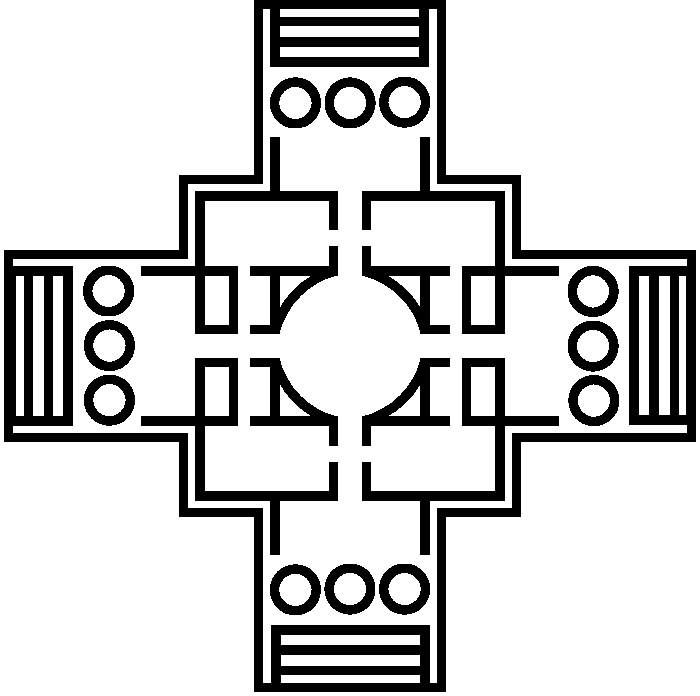
\includegraphics[height=\imagewidth]{figures/images/palladio-logo.pdf} \\ \acrshort{PCM}};
\node[above right=0.39*\vdistance and 0.5*\hdistance of system.center, tool] (java) {
\includegraphics[height=\imagewidth]{figures/images/java-logo.pdf} \\ Java};
\node[below left=0.66*\vdistance and 0.5*\hdistance of system.center, tool] (uml) {
\includegraphics[height=\imagewidth]{figures/images/uml-logo.pdf} \\ \acrshort{UML}};
\node[below right=0.66*\vdistance and 0.5*\hdistance of system.center, tool] (doors) {
\includegraphics[height=\imagewidth]{figures/images/doors-logo.png} \\ Doors};

\umlhuman{performance_engineer}{}{above left=0.5em and 0.75*\hdistance of pcm.center, anchor=center}{}{0.5}
\node[below=0em of performance_engineer.south, role] {Performance\\ Engineer};
\umlhuman{software_architect}{}{above left=0.5em and 0.75*\hdistance of uml.center, anchor=center}{}{0.5}
\node[below=0em of software_architect.south, role] {Software\\ Architect};
\umlhuman{software_developer}{}{above right=0.5em and 0.75*\hdistance of java.center, anchor=center}{}{0.5}
\node[below=0em of software_developer.south, role] {Software\\ Developer};
\umlhuman{requirements_engineer}{}{above right=0.5em and 0.75*\hdistance of doors.center, anchor=center}{}{0.5}
\node[below=0em of requirements_engineer.south, role] {Requirements\\ Engineer};

\draw[relation] (pcm) -- node[stereotype, sloped, above] (pcmjava) {\relatedtotext} (java);
\draw[relation] (uml) -- node[stereotype, sloped, above] (umlpcm) {\relatedtotext} (pcm);
\draw[relation] (uml) -- node[stereotype, sloped, above] (umljava) {\relatedtotext} (java);
\draw[relation] (doors) -- node[stereotype, sloped, above] (doorsjava) {\relatedtotext} (java);
\draw[relation] (uml) -- node[stereotype, sloped, pos=0.58, above] (umldoors) {\relatedtotext} (doors);

\draw[uses] (performance_engineer) -- node[stereotype, pos=0.32, above] {\usestext} (performance_engineer-|pcm.west);
\draw[uses] (software_architect) -- node[stereotype, pos=0.32, above] {\usestext} (software_architect-|uml.west);
\draw[uses] (software_developer) -- node[stereotype, pos=0.32, above] {\usestext} (software_developer-|java.east);
\draw[uses] (requirements_engineer) -- node[stereotype, pos=0.32, above] {\usestext} (requirements_engineer-|doors.east);

\draw[knows] ([yshift=1em]performance_engineer.east) to[bend left=20] node[stereotype, pos=0.6, above] {\knowsabouttext} ([xshift=1em]pcmjava.north west);
\draw[knows] ([yshift=1em]software_architect.east) to[bend left=20] node[stereotype, sloped, above] {\knowsabouttext} (umlpcm.north);
\draw[knows] ([yshift=-0.8em]software_architect.east) to[bend right=25] node[stereotype, below right=0.1em and 0.5em] {\knowsabouttext} ++(0.7*\hdistance, -0.2*\vdistance) to[bend right=40] (umljava.south west);
\draw[knows] ([yshift=1em]requirements_engineer.west) to[bend right=20] node[stereotype, sloped, above] {\knowsabouttext} ([xshift=0.5em]doorsjava.south);
\draw[knows] ([yshift=-0.8em]requirements_engineer.west) to[bend left=15] node[stereotype, pos=0.5, below left=0.3em and 0.5em] {\knowsabouttext} ++(-0.7*\hdistance, -0.2*\vdistance) to[bend left=22] (umldoors.south);

\end{tikzpicture}
